\cleardoublepage\chapter{Related Work}\label{sec:related_work}\minitoc\vspace{.5cm}\index{SotA}

The concept of multipath is well-established, and in this section we will explore existing multipath protocols, their characteristics, and highlight the unique aspects of our approach. 
Additionally, we will discuss the building block for the MTX as well as the use cases for the \ac{MTX} library. 
Finally, we will take a closer look at the design of the 5G system, with a specific focus on the Data Plane, to explain our plan for showcasing the multipath tunnel using the \ac{gptu} protocol.

\section{Tunneling}\index{Tunneling}
\todo{these following are my words, but do I need cite here?}
The concept of a network tunnel draws inspiration from its real-world counterpart, which refers to a confined pathway constructed to direct transportation between two points, separate from the surrounding terrain. 
In the physical sense, tunnels are often excavated deep beneath the earth's surface to bypass obstacles like mountains, rivers, or ocean channels.
In the realm of networking, a tunnel can be perceived as a direct network pathway that enables access to another network from the network to which it is currently connected. 
From an infrastructure standpoint, a tunnel serves as an abstraction layer that abstracts the actual traffic routing from the application and isolates the tunnel's traffic from public network traffic. 
This is typically achieved by encapsulating the application's data packets within the tunnel's packets, and then extracting the original data at the other end of the tunnel.
Many tunnel protocols exist for different purposes: IPv4/IPv6 tunnels to enable compatibility between exclusive networks \cite{rfc4380_Teredo_ipv6_tunnel_udp}, Secure Shell (SSH) - tunnel for remote access and data transfer \cite{rfc4251_ssh_protocol}, and \ac{VPN} tunneling - used for access other network from another network. 
\ac{VPN}s are frequently utilized to remotely access a private network, such as connecting to university's network from home. 
It also functions to conceal the origin of network traffic by making it appear as if it originates from the VPN server, which is useful for bypassing firewalls or restrictions applied by local network providers.
The traffic can also be encrypted to add an extra layer of protection while accessing networks over untrusted connections, like public WLAN provided by coffee shops.
Multiple VPN protocols are well-known and acknowledged, such as WireGuard, OpenVPN, IPsec, Cisco AnyConnect VPN, L2TP/IPsec, and SSTP (Secure Socket Tunneling Protocol). 
Each protocol carries its distinct philosophy, background, and intended area of application. 
MTX stood out by incorporating the multipath concept into its approach.

\section{Multipath Connection}\index{Multipath Connection}\label{sec:related_work:mp_connection}
Our primary emphasis is on establishing a connection between two points, irrespective of the number of physical transportation links.
% We will explore various protocols that implement the concept and make comparisons with our approach.
There are 2 approaches to utilize multiple links: managing multiple underlying connections created by existing protocols (\ac{MPTCP} with TCP), and creating a new multipath protocol (\ac{SCTP}).
Drawing inspiration from these protocols, our design of \ac{MTX} adopts a hybrid approach: a tunnel that transfers data over multiple UDP connections instead of maintaining TCP sessions. 
The tunnel data path comprises two primary logical stages: the data stage and the transport stage. 
The data stage handles session management, congestion control overhead, and other administrative tasks, enabling the transport stage to be constructed with wrappers over UDP sockets.
Unlike serving solely the caller, the multipath tunnel is designed to offer connection and flow management for multiple applications, enabling centralized resource management and scheduling.

\subsection{Multipath TCP}\label{sec:related_work:mp_connection:MPTCP}
% MultiPath TCP (MPTCP) is an effort towards enabling the simultaneous use of several IP-addresses/interfaces by a modification of TCP that presents a regular TCP interface to applications, while in fact spreading data across several subflows. Benefits of this include better resource utilization, better throughput and smoother reaction to failures. 

\ac{MPTCP} is is a major extension to TCP to decoupling the transport layer by utilizing multiple TCP-based sub flows \cite{Bonaventure_mptcp_decoupling}.
The protocol is showcased in both mobile and data center environments with distinct objectives. 
% In addition to enhancing data center performance by employing \ac{MPTCP}'s distributed load-balancing across multiple paths, the protocol also provides redundancy and effective congestion management capabilities \cite{raiciu_improving_nodate}.
\ac{MPTCP} enhances data center performance by employing \ac{MPTCP}'s distributed load-balancing across multiple paths, providing redundancy and effective congestion management capabilities \cite{raiciu_improving_nodate}.
In the context of mobile hand-over capability, \ac{MPTCP} helps maintain TCP sessions while the user equipment moves continuously. 
For instance, a smartphone can continue utilizing both LTE and Wi-Fi connections for a TCP session and predict the optimal route for transmitting most of the traffic. 
By monitoring the radio signal strength, it becomes possible to anticipate potential disruptions in the Wi-Fi connection or when a user enters a building and encounters a loss of cellular signal. 
The author argues that although maintaining two radios simultaneously consumes more power, it can potentially reduce the time required to establish new connections and transmit data \cite{paasch_multipath_2014}.

\begin{figure}[H]
	\centering
	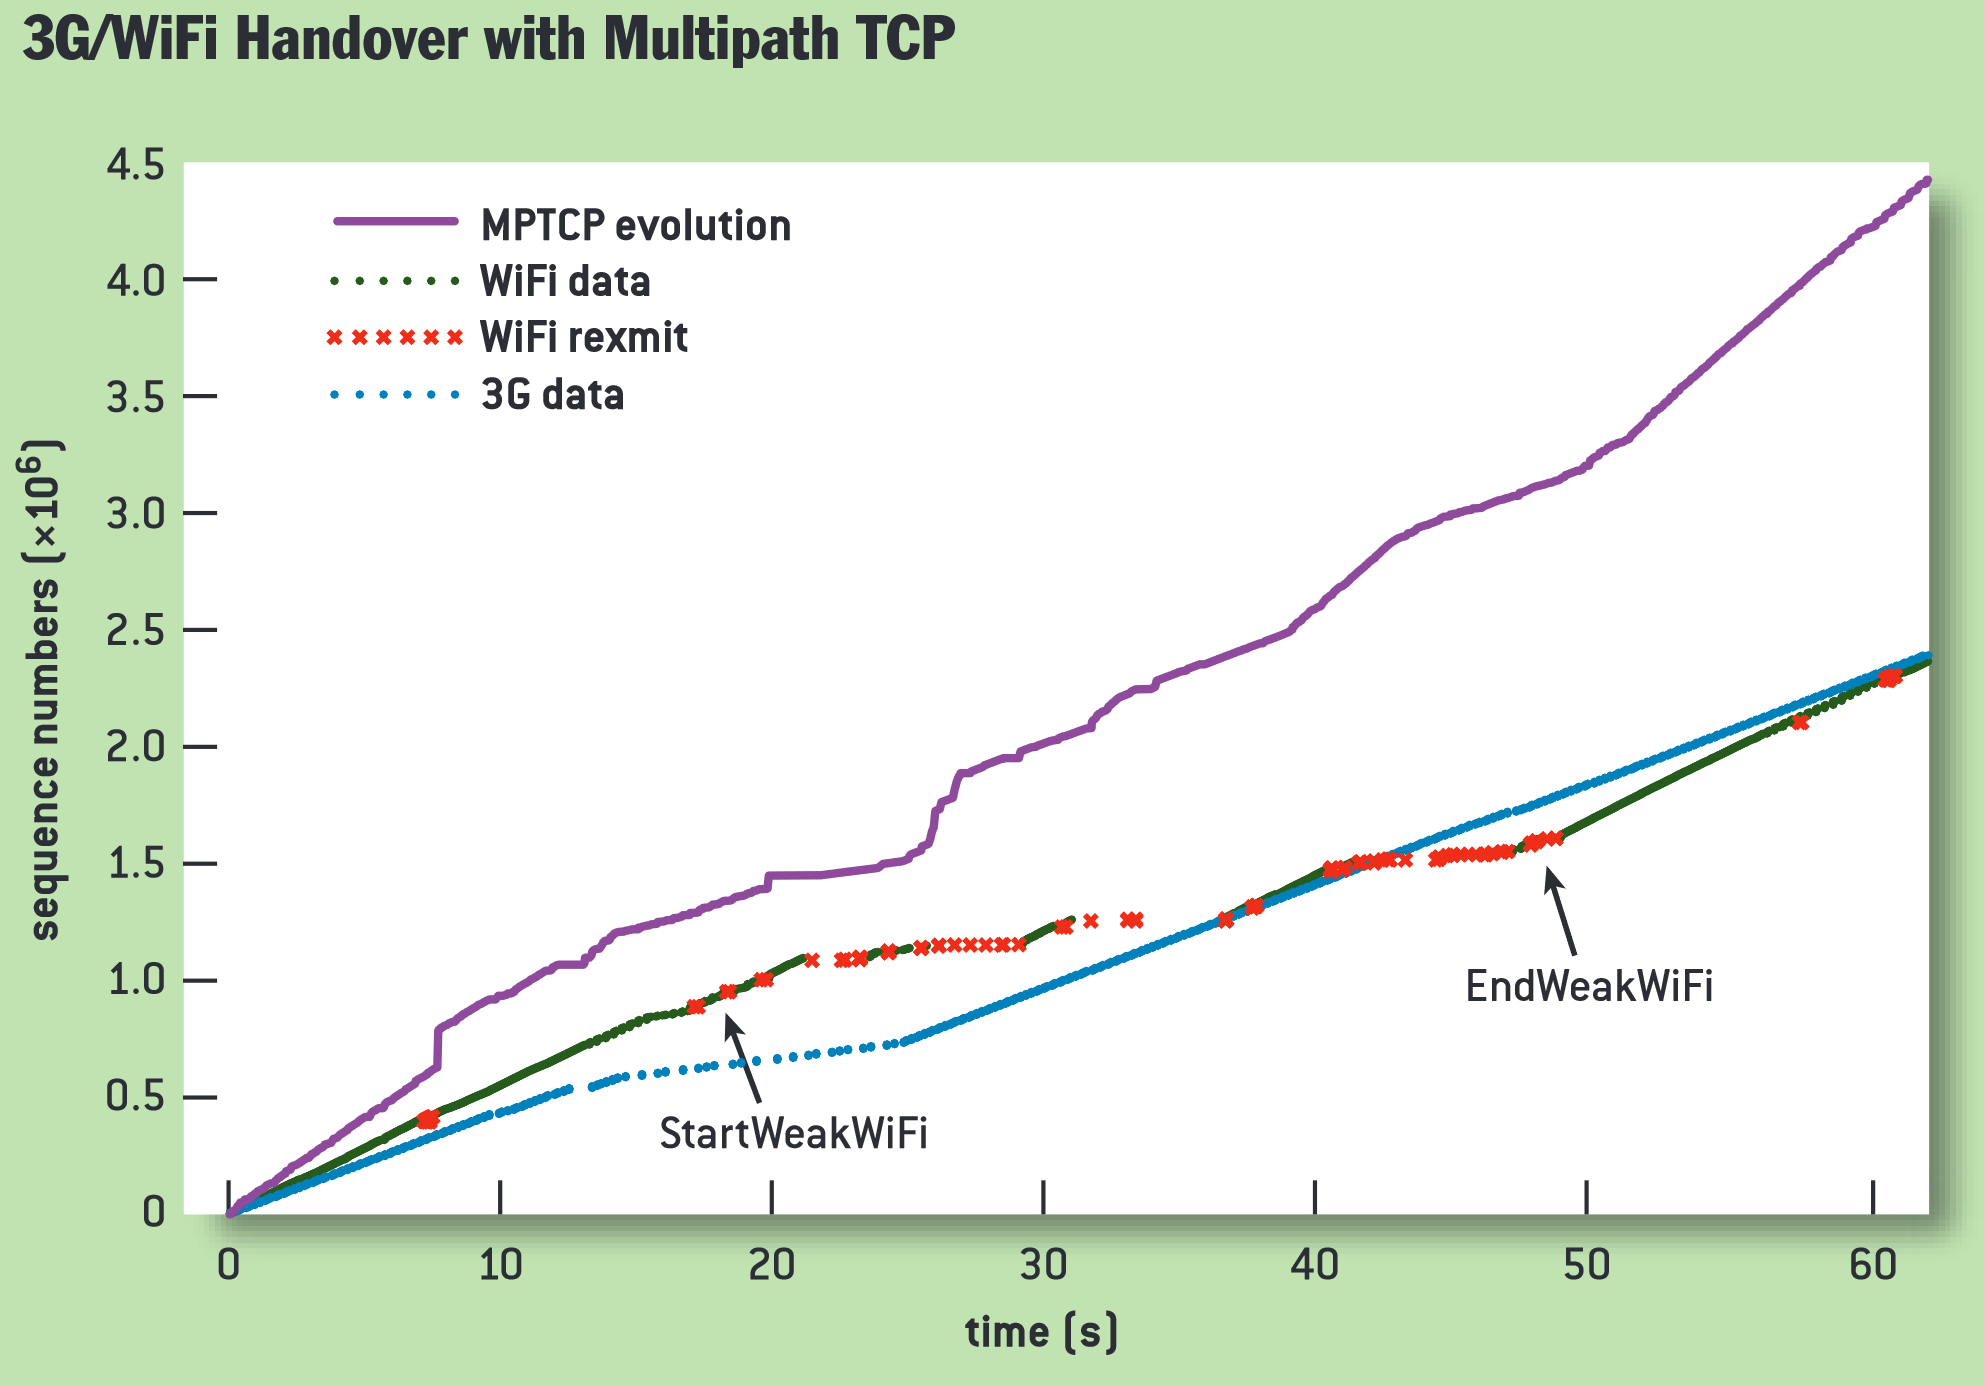
\includegraphics[width=0.7\textwidth]{resources/images/3G_WiFi_Handover_with_Multipath_TCP.PNG}
	\caption{3G/WiFi Handover with Multipath TCP \cite{paasch_multipath_2014}. The MPTCP connection (in violet) persists despite of WiFi and 3G's unreliable connections. A weak WiFi signal can be indicative of the device moving beyond the coverage range of the router. The command \textit{REXMIT} changes the time-out value for each packet which is used for retransmitting packet. This indicates the TCP connection was trying to retransmit over the weakening WiFi connection.}
    \label{fig:related_work:3G_WiFi_Handover_with_Multipath_TCP}
\end{figure}

\subsection{Stream Control Transmission Protocol}\label{sec:related_work:mp_connection:SCTP}
\ac{SCTP} introduces multiple addresses to the transport layer, which serves as failover or simultaneous sub-connection.
Unlike \ac{MPTCP}, existing internet's infrastructure such as firewalls, routers were not designed to handle \ac{SCTP}'s packets and thus severely limits usage of the protocol \cite{paasch_multipath_2014}. 
Notably, \ac{SCTP} is used in 5G core design for transmitting messages in Control plane.

\begin{figure}[H]
	\centering
	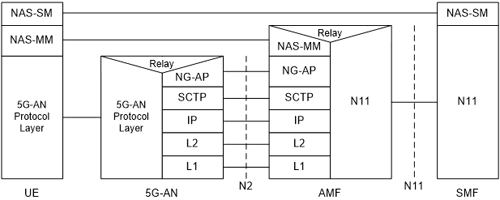
\includegraphics[width=0.8\textwidth]{resources/images/3gpp_5g_part_of_control_plane_protocol.png}
	\caption{3GPP: Control Plane protocol stack between the UE, the 5G-AN, the AMF and the SMF \cite{3gpp_5g_system_overview}}
    \label{fig:related_work:3gpp_5g_part_of_control_plane_protocol}
\end{figure}


\section{Current 5G Deployment: Multipath in Action}\index{Current 5G Deployment: Multipath in Action}
5G services and functions are designed to be deployed in containers and virtual machines, often on server-grade general purpose computers.
These components are categorized into two groups: the Control plane and the Data plane (\Cref{fig:related_work:Non_Roaming_5G_System_Architecture_in_reference_point_representation}).

\begin{figure}[H]
	\centering
	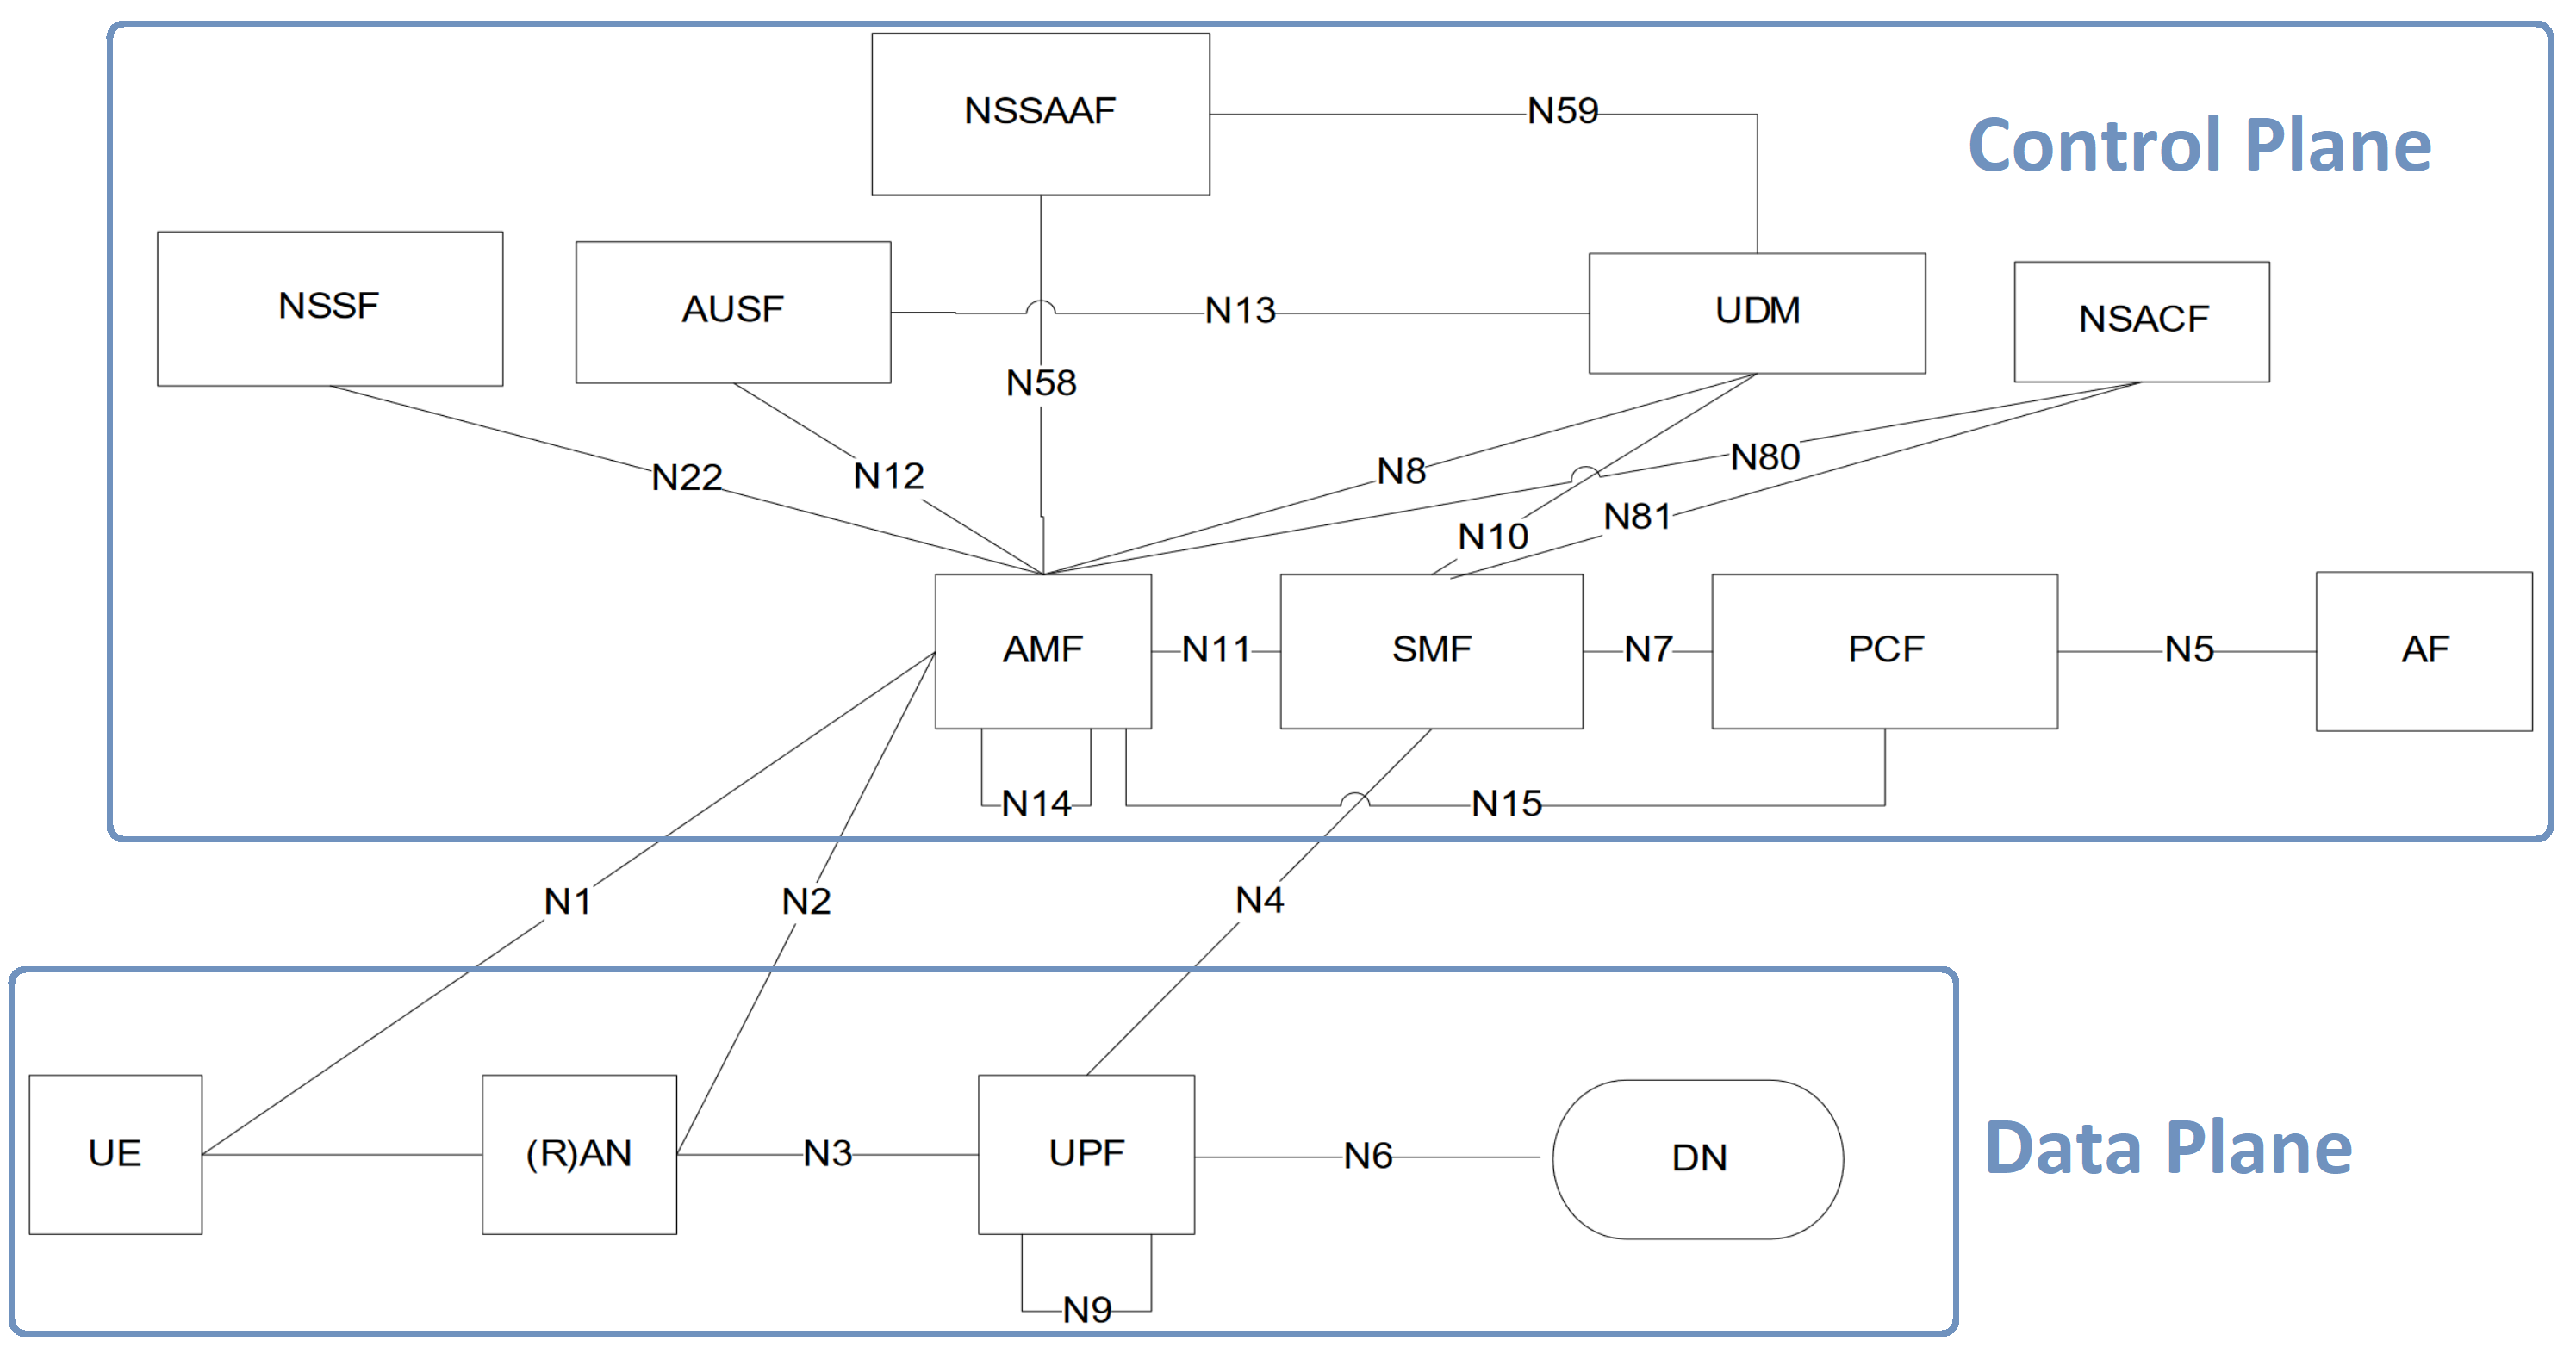
\includegraphics[width=1.0\textwidth]{resources/images/Non_Roaming_5G_System_Architecture_in_reference_point_representation.png}
	\caption{Adapted from 3GPP specification: Data and Control Plane in 3GPP's Non-Roaming 5G System Architecture in reference point representation \cite{3gpp_5g_system_architect_spec_release_18}}
	\label{fig:related_work:Non_Roaming_5G_System_Architecture_in_reference_point_representation}
\end{figure}

As mentioned in \Cref{sec:related_work:mp_connection:SCTP}, the control plane uses \ac{SCTP} protocol with multipath support for its internal communication.
For the Data Plane, while the \ac{gptu} protocol does not have a built-in feature equivalent to multipath, vendors have developed their own data plane technology stack to achieve high performance.
\ac{NEC} demonstrated its containerized \ac{UPF} solution's capability by handling 640Gbps bandwidth on 1 single 2x32 cores server \cite{nec_upf_whitepaper}.
\ac{dpdkpage} library was used to forward the enormous data flows.
\ac{ZTE} offers hardware platforms and software stack that use a combination of \ac{dpdkpage}, \ac{sriov} and hardware acceleration technology to support a wide range of bandwidth capacity from 5Gbps to 200Gbps \cite{zte_upf_full_whitepaper}, and up to 462Gbps in a test scenario in cooperation with Intel \cite{zte_5g_core_upf_impl}.

Our \ac{MTX} library is positioned as an alternative to packet handling components based on \ac{dpdkpage} and \ac{sriov}. 
In the subsequent sections, we will introduce these two technologies and highlight the potential advantages offered by our solution. \todo{I keep this text since MTX offers no perf improvement but usability and compability}

\section{MTX Enhancement for 5G Data Plane}\index{MTX Enhancement for 5G Data Plane}
\label{sec:related_work:5g_dataplane_enhancement}
In \Cref{fig:related_work:5g_dp_enhancement} we describe how data is moved between \ac{UE} and \ac{DN}, based on 3GPP specification and various sources.
A \ac{PDU} session is established to create a logical data path between \ac{UE} and \ac{UPF}.
This \ac{PDU} logical session runs on top of several transporting protocol.
Radio Bearer (RB) is the channel to move user data and control data between UE and radio equipment.
The \ac{eCPRI} protocol connects front-haul network and moves user data, controlling and management data, and synchronization data flows between DU and RU \cite{eCPRI_spec}.
\ac{gptu} connection - often called \textit{tunnel} - helps transferring user data between middle-haul and back-haul networks in UDP packets.
Data in different categories receives forwarding treatment differently, depends on the priority, subscription, ... 
This is managed by splitting the data into streams (called \ac{QoS} Flow, marked with QoS Flow Identification (QFI)), each is governed with different rule set (QoS rules).
\\

Two potential improvements can be applied to the 5G network with out MTX tunnel:
\begin{itemize}
    \item N6 connection between UPF (also N9 i.e between UPF-E and UPF-C) and Data network: enhanced by prioritized, flow-aware, high bandwidth multipath tunnel. 
	To meet differentiated SLA requirements for latency, bandwidth and reliability, UPF needs to be deployed at different positions including central DC, regional DC, edge DC and campus DC. 
	MTX can help saturating physical links coup with support large number of UEs.
    \item 5G user plane:  
	The back-haul N3 connection between gNodeB-UPF, and mid-haul F1 connection between gNodeB-CU and -DU relied on message-based protocol \ac{gptu} (the character "U" means "user data tunneling") to relay traffic within a PDP session.
\end{itemize}

% \begin{figure}[H]
% 	\centering
% 	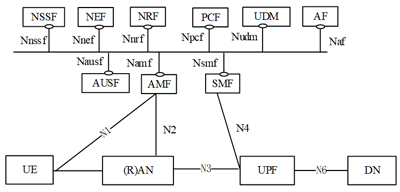
\includegraphics[width=0.8\textwidth]{resources/images/3gpp_5g_system_overview.png}
% 	\caption{3GPP's 5G System Overview \cite{3gpp_5g_system_overview}}
%     \label{fig:related_work:3gpp_5g_system_overview}
% \end{figure}

\begin{figure}[H]
	\centering
	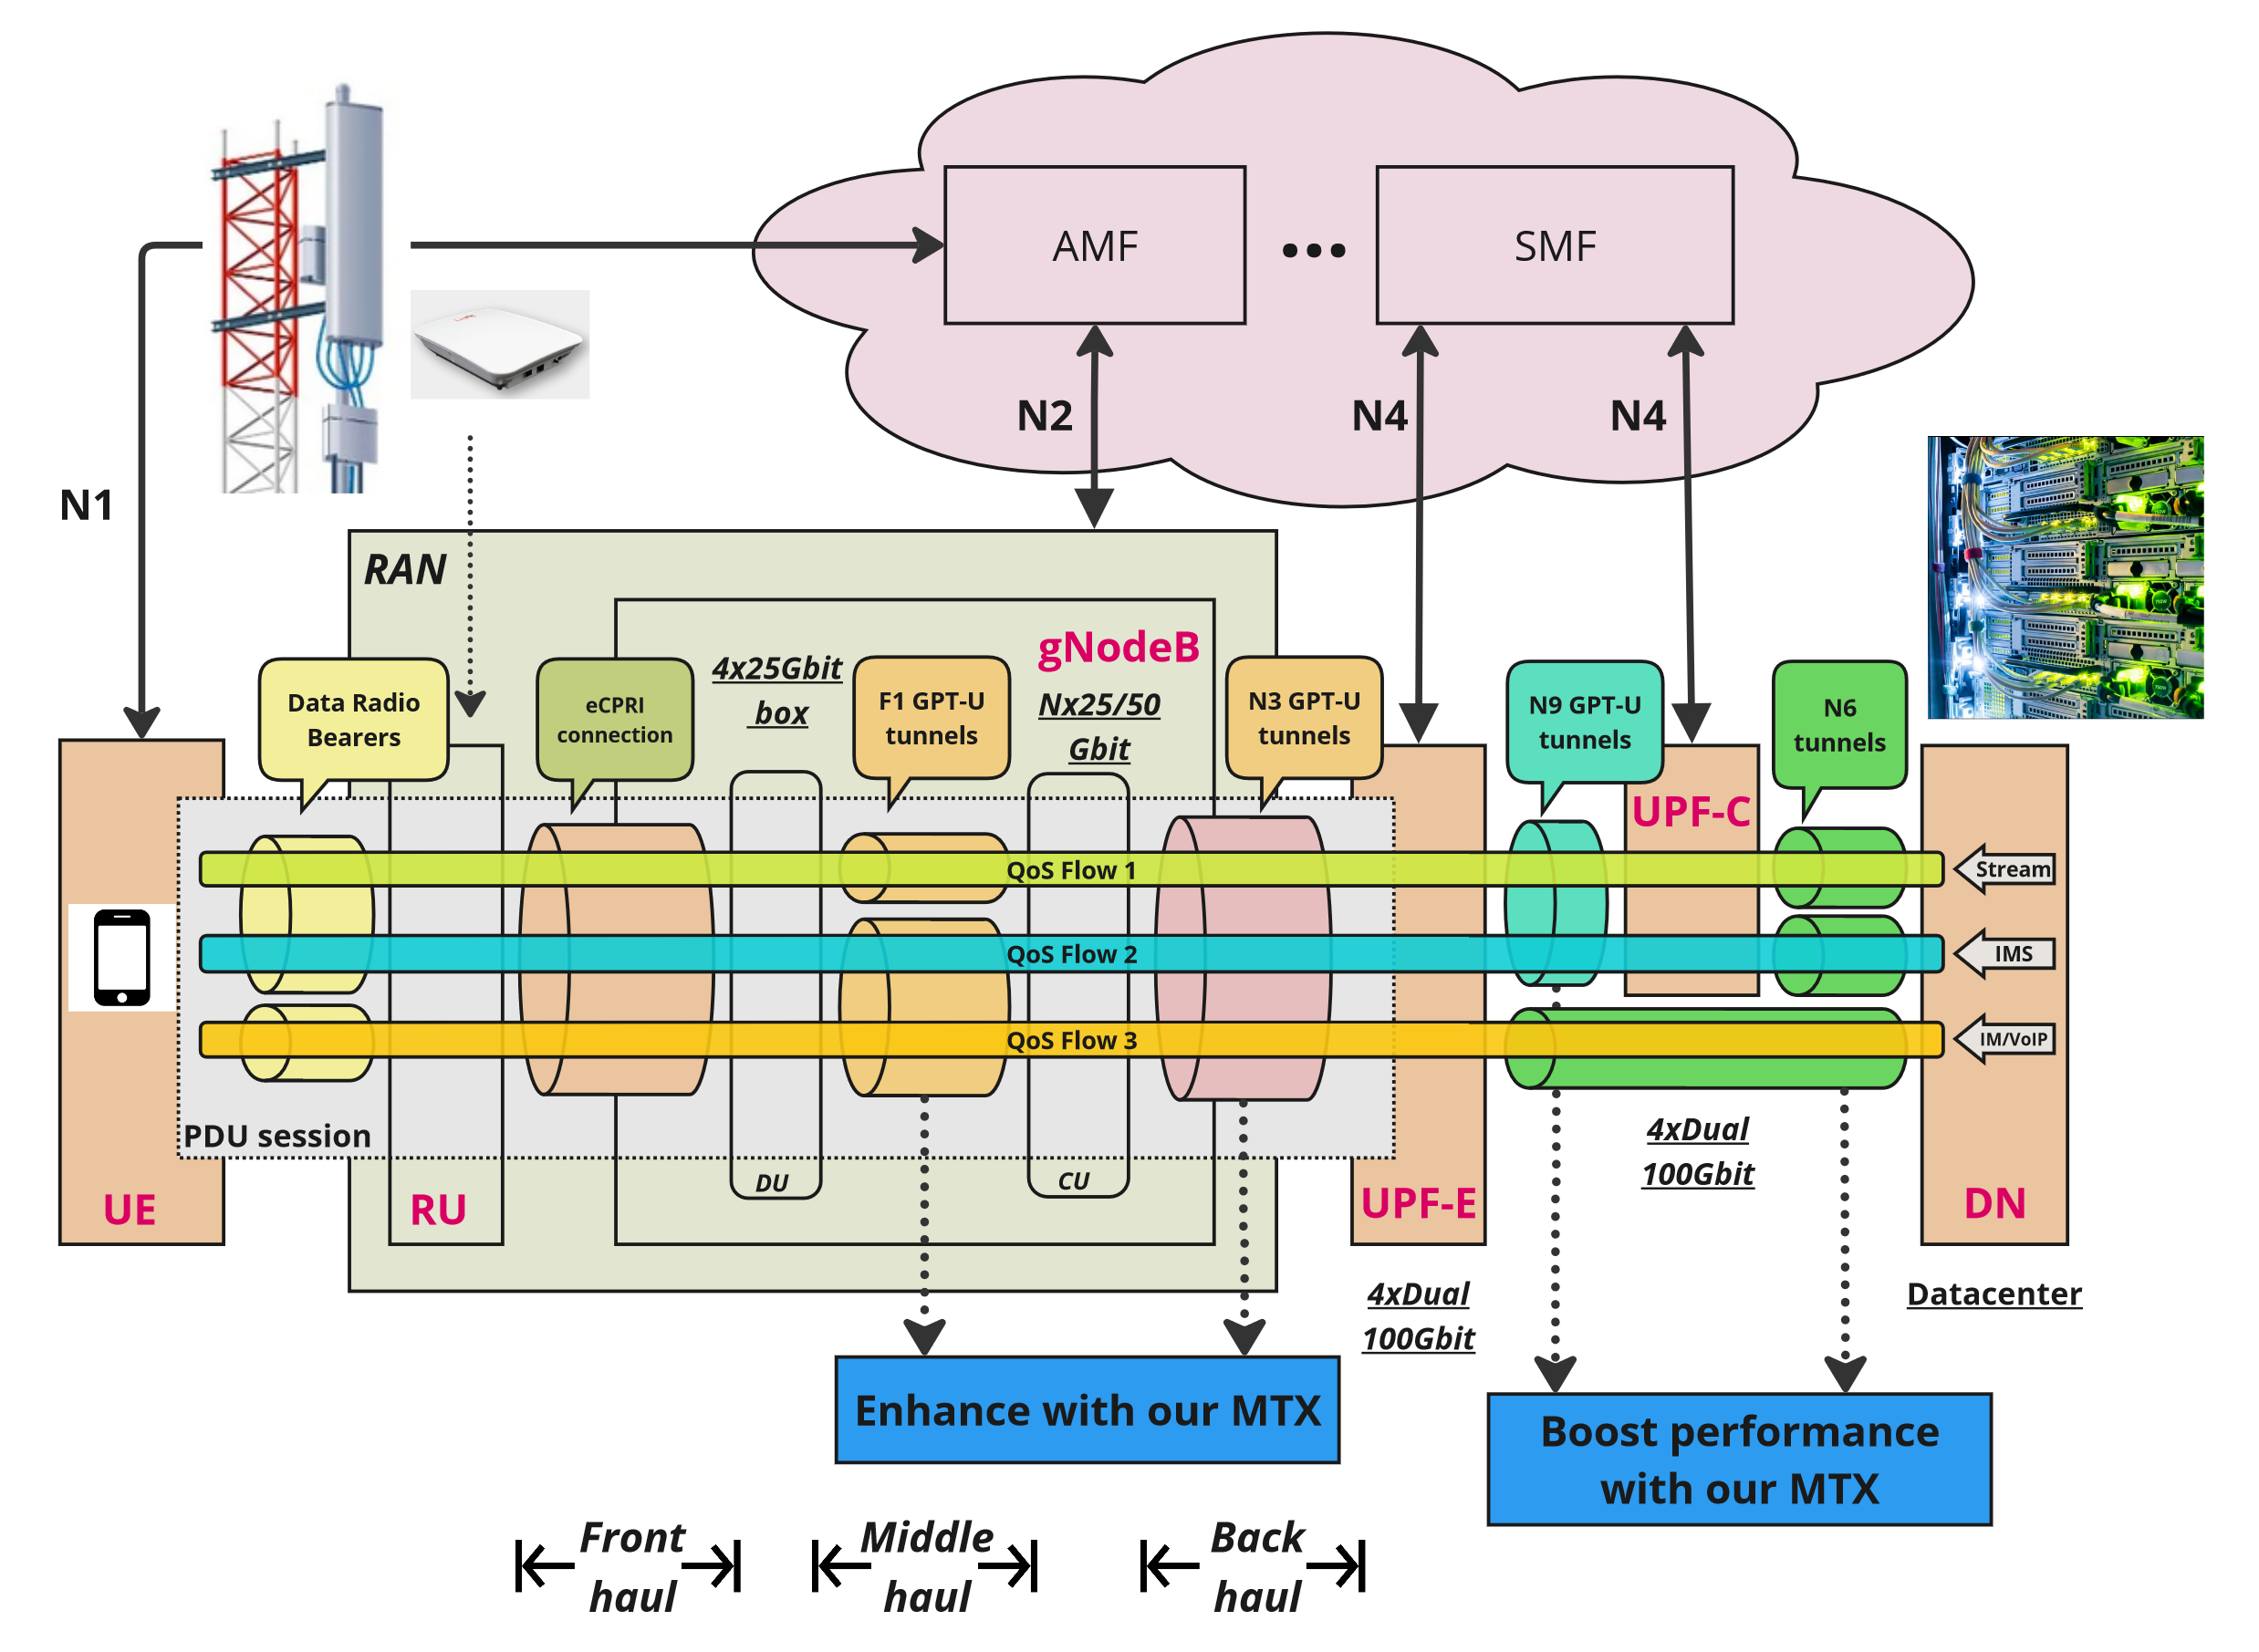
\includegraphics[width=1.0\textwidth]{resources/images/5g_dp_enhancement.PNG}
	\caption{5G Data Plane overview. The MTX library will be used as the building block for the GPT-U enhancement, which bring multipath capability to the protocol. Raw MTX can also be used to help connecting UPF and DN over multiple links.}
    \label{fig:related_work:5g_dp_enhancement}
\end{figure}

In actual deployed systems, \ac{gptu} tunnels are typically established and configured professionally on top of multiple links that are aggregated and managed by a software stack, for instance \ac{dpdkpage} and \ac{sriov}, which involve costly software and (powerful and specifically chosen) hardware that lack flexibility.
The alternative, open source implementations usually suffers from performance losses due to inefficiency, as noted in Open5GS discussion \cite{open5gs_github_udp_perf_cap}\cite{open5gs_github_dpdk}.
\\

One of the project's goals is to tackle the performance and usability issues by exploring the development of a straightforward yet robust multipath tunnel capable of functioning in both physical and virtual environments. 
To ensure ease of maintenance and facilitate compatibility with other protocols, we aim for a tunnel code base that remains simple and minimizes the need for extensive modifications, which is why \ac{xdppage} has been selected as the preferred transport method.
For the testing phase, we have chosen the \ac{gptu} protocol due to its diverse range of requirements that can be supported by MTX, including flow-awareness, high throughput, low latency, and a comprehensive set of configuration options.


% \begin{figure}[H]
% 	\centering
% 	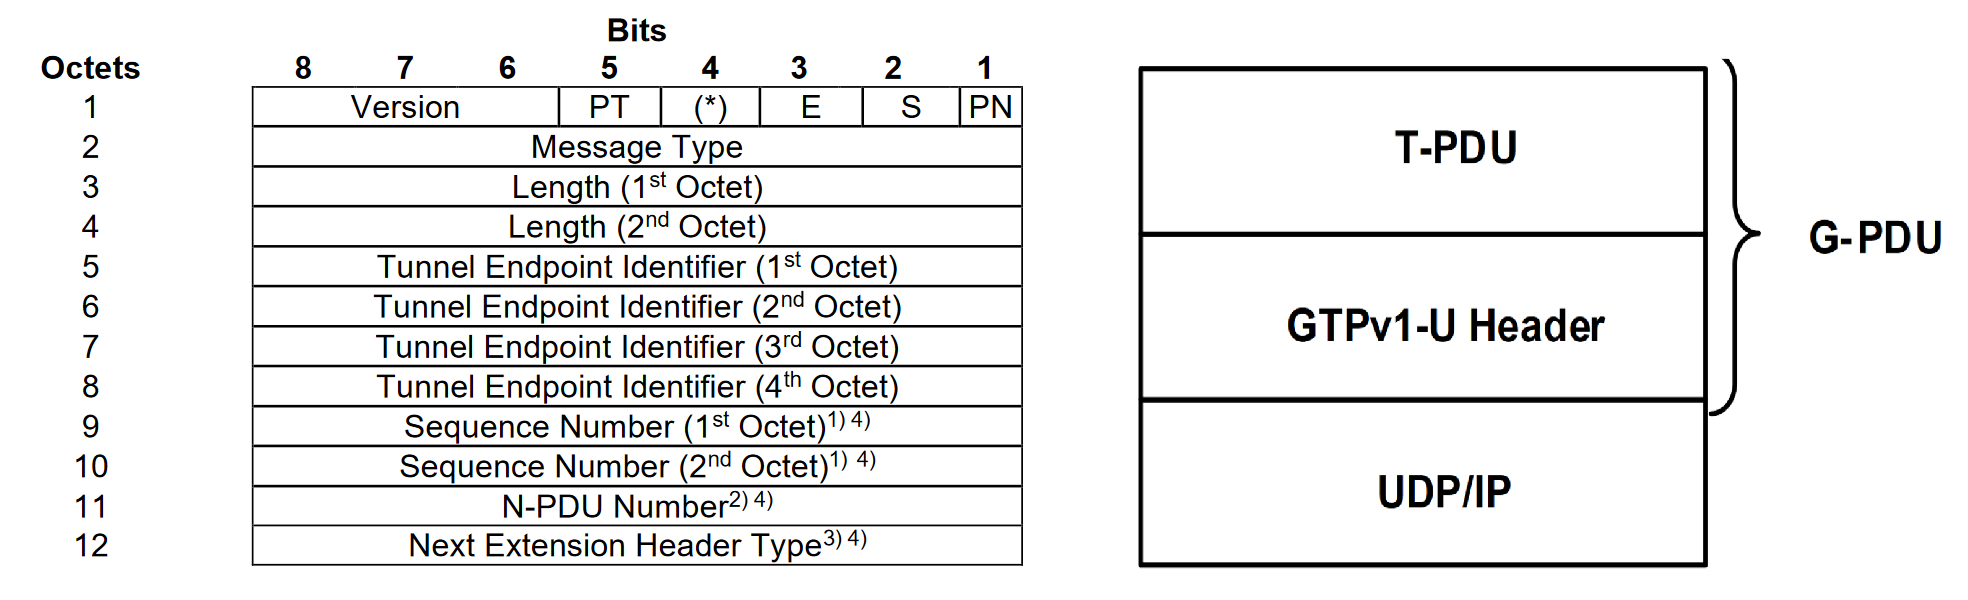
\includegraphics[width=1.0\textwidth]{resources/images/gptu_header_and_gpdu_stack.PNG}
% 	\caption{3GPP: GPT-U header and G-PDU Protocol Stack built on top of UDP/IP protocol \cite{3gpp_gptu}}
%     \label{fig:related_work:gptu_header_and_gpdu_stack}
% \end{figure}

